\begin{usecase}{Receive Event Notifications}
  \ucbasicinfo{High}{Regular}
  \ucshortdescription{Users receive notifications about upcoming events.}
  \uctrigger{The UC is triggered when the chosen time of an event's reminder has arrived.}
  \ucactors{User}{None}
  \ucpreconditions{User must be logged into the system and have set a reminder for a specific event.}
  \ucrelationships{N/A}{N/A}{N/A}
  \ucinputsoutputs{
    \begin{itemize}
      \item \textbf{Event reminders/alerts} (Source: User)
    \end{itemize}
  }{
    \begin{itemize}
      \item \textbf{Local notifications displayed to the user.} (Destination: System)
    \end{itemize}
  }
  \ucmainflow{
    \begin{enumerate}
      \item The system iterates over all events with reminders set.
      \item For each event, a local notification is scheduled to remind the user.
    \end{enumerate}
  }
  \ucalternateflows{
    \begin{itemize}
      \item \textbf{If the user denies notification permissions, notifications cannot be sent.}
    \end{itemize}
  }
  \ucexceptions{
    \begin{itemize}
      \item \textbf{System error or failure to schedule notifications.}
    \end{itemize}
  }
  \ucconclusion{The system schedules local notifications for all events with reminders.}
  \ucpostconditions{Notifications are displayed to the user at the appropriate time.}
  \ucspecialrequirements{Notification permissions must be granted by the user.}
  \ucbusinessrules{The system must ensure notifications are scheduled accurately and on time.}
\end{usecase}

\begin{figure}[!h]
  \centering
  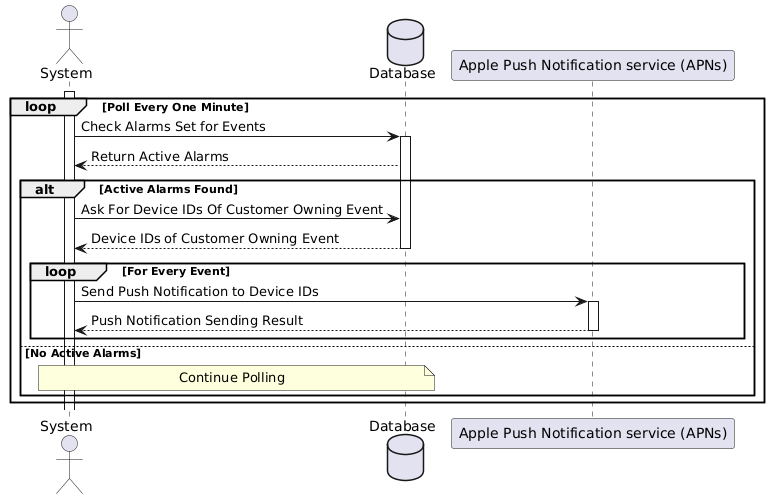
\includegraphics[width=\textwidth]{images/docs/diagrams/sequence-diagrams/all-sequence-diagrams/Receive Event Notifications.png}
  \caption{Receive Event Notifications Sequence Diagram}
  \label{fig:seq/receive-event-notifications}
\end{figure}

The ``Receive Event Notifications Sequence Diagram'', shown in \textbf{Figure~\ref{fig:seq/receive-event-notifications}}, depicts the flow of how local event reminders are scheduled and delivered to the user. When the user sets a reminder for a calendar event, it is saved using EventKit. The application periodically retrieves all upcoming events with reminders from EventKit and schedules local notifications for each of them via the iOS notification system. At the scheduled time, iOS automatically triggers the corresponding local notification, ensuring the user is reminded promptly. This flow assumes the user has granted the necessary notification permissions and is logged into the application.
